\section{Partonymy/Meronymy}
\label{sec:Partonymy}
%%%%%%%%%%%%%%%%%%%%%%%%%%%%%%%%%%%%%%%%%%%%%%%%%%%%%%%%
\begin{figure}[h!]
\begin{center}
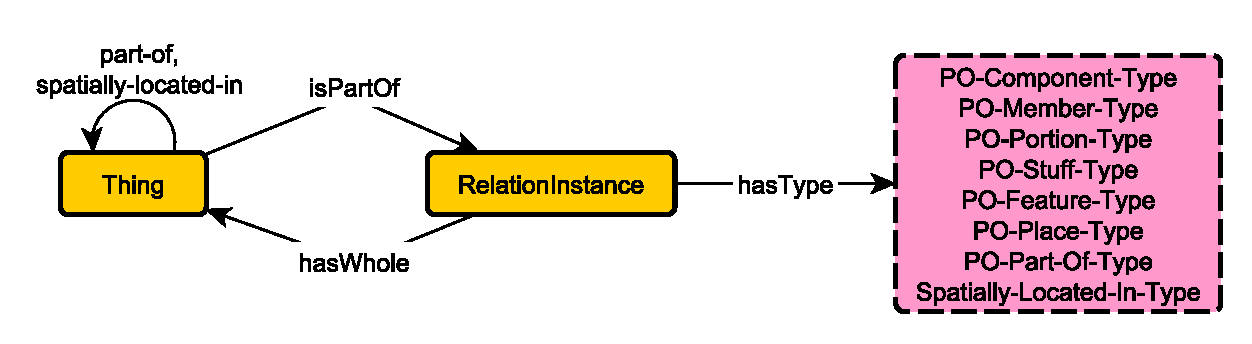
\includegraphics[width=.7\textwidth]{figures/partonymy}
\end{center}
\caption{Schema Diagram for Partonymy.}
\label{fig:Partonymy}
\end{figure}
\subsection{Summary}
\label{sum:Partonymy}
%%%%%%%%%%%%%%%%%%%%%%%%%%%%
Part-whole relations are of fundamental importance for how we organize concepts. This pattern follows an approach laid out by Winston in his 1987 landmark paper on ``A Taxonomy of Part-Whole Relations'' \cite{citeulike:171338} which was based on linguistic considerations, but also provided for logical characterizations and axiomatics, and, as such, inform the pattern.

Essentially, we distinguish between different, interacting partonomies. For example, a component may be part of an engine, which is part of a plane, which belongs to a fleet. These are all part-hood relationships, but they are not transitive.

%%%%%%%%%%%%%%%%%%%%%%%%%%%%%%%%%%%%%%%%%%%%%%%%%%%%%%%%
\subsection{Axiomatization}
\label{axs:Partonymy}
%%%%%%%%%%%%%%%%%%%%%%%%%%%%
\begin{align}
\poComObj \circ \poComObj &\sqsubseteq \poComObj \label{ax:trans1}\\
\poMemCol \circ \poMemCol &\sqsubseteq \poMemCol \\
\poPorMas \circ \poPorMas &\sqsubseteq \poPorMas \\
\poStuObj \circ \poStuObj &\sqsubseteq \poStuObj \\
\poFeaAct \circ \poFeaAct &\sqsubseteq \poFeaAct \\
\poPlaAre \circ \poPlaAre &\sqsubseteq \poPlaAre \label{ax:trans6}\\
\text{AsymmetricObjectProperty}&(\poComObj) \label{ax:asym1}\\
\text{AsymmetricObjectProperty}&(\poMemCol)\\
\text{AsymmetricObjectProperty}&(\poPorMas)\\
\text{AsymmetricObjectProperty}&(\poStuObj)\\
\text{AsymmetricObjectProperty}&(\poFeaAct)\\
\text{AsymmetricObjectProperty}&(\poPlaAre) \label{ax:asym6}\\
\poComObj &\sqsubseteq \partOf \label{ax:subpof1}\\
\poMemCol &\sqsubseteq \partOf\\
\poPorMas &\sqsubseteq \partOf\\
\poStuObj &\sqsubseteq \partOf\\
\poFeaAct &\sqsubseteq \partOf\\
\poPlaAre &\sqsubseteq \partOf \label{ax:subpof6}\\
\spatialLocIn \circ \spatialLocIn &\sqsubseteq \spatialLocIn \label{ax:transloc}\\
\text{ReflexiveObjectProperty}&(\spatialLocIn)\\
\poComObj\circ\spatialLocIn&\sqsubseteq \spatialLocIn \label{ax:spatial1}\\
\spatialLocIn\circ \poComObj&\sqsubseteq\spatialLocIn\\
\poMemCol\circ\spatialLocIn&\sqsubseteq \spatialLocIn\\
\spatialLocIn\circ \poMemCol&\sqsubseteq\spatialLocIn\\
\poPorMas\circ\spatialLocIn&\sqsubseteq \spatialLocIn\\
\spatialLocIn\circ \poPorMas&\sqsubseteq\spatialLocIn\\
\poStuObj\circ\spatialLocIn&\sqsubseteq \spatialLocIn\\
\spatialLocIn\circ \poStuObj&\sqsubseteq\spatialLocIn\\
\poFeaAct\circ\spatialLocIn&\sqsubseteq \spatialLocIn\\
\spatialLocIn\circ \poFeaAct&\sqsubseteq\spatialLocIn\\
\poPlaAre\circ\spatialLocIn&\sqsubseteq \spatialLocIn\\
\spatialLocIn\circ \poPlaAre&\sqsubseteq\spatialLocIn\\
\textsf{Po-Component-Type}         &\sqsubseteq \textsf{RelationInstance} \\
\textsf{Po-Member-Type}            &\sqsubseteq \textsf{RelationInstance} \\
\textsf{Po-Portion-Type}           &\sqsubseteq \textsf{RelationInstance} \\
\textsf{Po-Stuff-Type}             &\sqsubseteq \textsf{RelationInstance} \\
\textsf{Po-Feature-Type}           &\sqsubseteq \textsf{RelationInstance} \\
\textsf{Po-Place-Type}             &\sqsubseteq \textsf{RelationInstance} \\
\textsf{Po-Part-Of-Type}           &\sqsubseteq \textsf{RelationInstance} \\
\textsf{Spatially-Located-In-Type} &\sqsubseteq \textsf{RelationInstance}
\end{align}

%%%%%%%%%%%%%%%%%%%%%%%%%%%%%%%%%%%%%%%%%%%%%%%%%%%%%%%%
\subsection{Explanations}
\label{exp:Partonymy}
%%%%%%%%%%%%%%%%%%%%%%%%%%%%
\begin{enumerate}
\item Transitivity.
\item Transitivity.
\item Transitivity.
\item Transitivity.
\item Transitivity.
\item Transitivity.
\item Asymmetric Object Property.
\item Asymmetric Object Property.
\item Asymmetric Object Property.
\item Asymmetric Object Property.
\item Asymmetric Object Property.
\item Asymmetric Object Property.
\item Subclass.
\item Subclass.
\item Subclass.
\item Subclass.
\item Subclass.
\item Subclass.
\item Transitivity.
\item Reflexive Object Property.
\item Role Chain: the concatenation of \poComObj{} and \spatialLocIn{} is \spatialLocIn{}.
\item Role Chain: the concatenation of \spatialLocIn{} and \poComObj{} is \spatialLocIn{}.
\item Role Chain: the concatenation of \poMemCol{} and \spatialLocIn{} is \spatialLocIn{}.
\item Role Chain: the concatenation of \spatialLocIn{} and \poMemCol{} is \spatialLocIn{}.
\item Role Chain: the concatenation of \poPorMas{} and \spatialLocIn{} is \spatialLocIn{}.
\item Role Chain: the concatenation of \spatialLocIn{} and \poPorMas{} is \spatialLocIn{}.
\item Role Chain: the concatenation of \poStuObj{} and \spatialLocIn{} is \spatialLocIn{}.
\item Role Chain: the concatenation of \spatialLocIn{} and \poStuObj{} is \spatialLocIn{}.
\item Role Chain: the concatenation of \poFeaAct{} and \spatialLocIn{} is \spatialLocIn{}.
\item Role Chain: the concatenation of \spatialLocIn{} and \poFeaAct{} is \spatialLocIn{}.
\item Role Chain: the concatenation of \poPlaAre{} and \spatialLocIn{} is \spatialLocIn{}.
\item Role Chain: the concatenation of \spatialLocIn{} and \poPlaAre{} is \spatialLocIn{}.
\item Subclass.
\item Subclass.
\item Subclass.
\item Subclass.
\item Subclass.
\item Subclass.
\item Subclass.
\item Subclass.
\end{enumerate}

%%%%%%%%%%%%%%%%%%%%%%%%%%%%%%%%%%%%%%%%%%%%%%%%%%%%%%%%
\subsection{Competency Question}
\label{cqs:Partonymy}
%%%%%%%%%%%%%%%%%%%%%%%%%%%%
\begin{enumerate}[CQ1.]
\item Is the Everglades part of Florida?
\item Is the plane in the Warehouse?
\item What are all engine components?
\item Is he part of the family?
\end{enumerate}

\newpage
%%%%%%%%%%%%%%%%%%%%%%%%%%%%%%%%%%%%%%%%%%%%%%%%%%%%%%%%
% End Section
%%%%%%%%%%%%%%%%%%%%%%%%%%%%%%%%%%%%%%%%%%%%%%%%%%%%%%%%
%%%%%%%%%%%%%%%%%%%%%%%%%%%%%%%%%%%%%%%%%%%%%%%%%%%%%%%%